\documentclass[a4paper,10pt,twoside]{article}

\usepackage[utf8]{inputenc}
\usepackage{enumitem}
\usepackage{moreenum}
\usepackage{graphicx}
\usepackage{fancyref}
\usepackage{multirow}
\usepackage{hyperref}
\usepackage[normalem]{ulem}
\usepackage[title]{appendix}
\usepackage{listings}

\textheight25.0cm
\textwidth16cm
\topmargin-.5cm
\oddsidemargin 0.cm
\evensidemargin 0.cm
\headheight0.5cm
\headsep0.cm
\footskip0.7cm
%\footheight2.5cm
\marginparwidth1.2cm
\marginparsep0.3cm

%%%%%%%%%%%%%%%%%%%%%%%%%%%%%%%%%%%%%%%%%%%%%%%%% END of HEADER

\title{DAVAÏ User Guide}
\author{A. Mary}
\date{\today}

\pdfinfo{%
  /Title    (Ugr)
  %/Author   (A. mary)
  /Creator  ()
  /Producer ()
  /Subject  ()
  /Keywords ()
}

\begin{document}
\maketitle

\tableofcontents
\vspace{1cm}
\newpage


DAVAÏ embeds the whole workflow from the source code to the green/red light validation status: fetching sources from Git, building executables, running test cases, analysing the results and displaying them on a dashboard.

For now, the only build system embedded is \texttt{gmkpack}, but we expect other systems to be plugged when required. The second limitation of this version is that the starting point is still an IAL Git reference only. The next version of the DAVAÏ system will include multi-projects/repositories fetching, using the \textit{\texttt{bundle}} concept as starting point.

The dimensioning of tests (grid sizes, number of observations, parallelization...) is done in order to conceal representativity and execution speed. Therefore, in the general usecases, the tests are supposed to run on HPC. A dedicated usecase will target smaller configurations to run on workstation (not available yet).\\

An accessible source code forge is set within the ACCORD consortium to host the central repository on which updates and releases are published, and where integration requests will be posted, reviewed and monitored.
\begin{center}
 \rule{8cm}{1pt}
\end{center}

By the way: DAVAI stands for \textit{``\textbf{D}evice \textbf{A}iming at the \textbf{VA}lidation of \textbf{I}AL\footnote{IAL = \textbf{I}FS-\textbf{A}rpege-\textbf{L}AM}''}

\newpage
\section{TUTORIAL: Test an IAL development} 
\subsection{Create your branch, containing your modifications}
To use DAVAÏ to test your contribution to the next development release, you need to have your code in a Git branch starting from the latest official release (e.g. \texttt{CY48T1} tag for contributions to 48T2, or \texttt{CY49} tag for contributions to 49T1).

\noindent In the following the example is taken on a contribution to 48T2:
\begin{enumerate}[label=(\greek*)]
 \item In your repository (e.g. \texttt{$\sim$/repositories/arpifs} -- make sure it is clean with \texttt{git status} beforehand), create your branch:\\
 \texttt{git checkout -b \textit{<my\_branch>} [\textit{<starting\_reference>}]}\\
 (e.g. \texttt{git checkout -b mary\_CY48T1\_cleaning CY48T1})\\
 \underline{Note:} it is strongly recommended to have explicit branch names with regards to their origin and their owner, hence the legacy branch naming syntax \texttt{<user>\_<CYCLE>\_<purpose\_of\_the\_branch>}
 \item Implement your developments in the branch.\\
 \textit{It is recommended to find a compromise between a whole development in only one commit, and a large number of very small commits (e.g. one by changed file).} In case you then face compilation or runtime issues then, but only if you haven't pushed it yet, you can \textit{amend}\footnote{\texttt{git commit --amend}} the latest commit to avoid a whole series of commits just for debugging purpose.\\
 \underline{Note:} DAVAÏ is currently able to include non-committed changes in the compilation and testing. However, in the next version based on \textit{bundle}, this might not be possible anymore.
\end{enumerate}


\subsection{Run tests} 
\subsubsection{Setup your experiment}
\begin{enumerate}[label=(\alph*)]
 \item Create your experiment, specifying which version of the tests you want to use:\\
 \texttt{davai-new\_xp \textit{<my\_branch>} -v \textit{<tests\_version>}}\\
 (e.g. \texttt{davai-new\_xp mary\_CY48T1\_cleaning -v DV48T1})\\
 $\hookrightarrow$ An experiment with a unique experiment ID is created and prompted as output of the command, together with its path. 
 \begin{itemize}
  \item to know what is the version to be used for a given development:\\
  \href{https://github.com/ACCORD-NWP/DAVAI-tests/wiki}{https://github.com/ACCORD-NWP/DAVAI-tests/wiki}
  \item see \texttt{davai-new\_xp -h} for more options on this command
  \item see Appendix~\ref{sect:tests_versioning} for a more comprehensive approach to tests versioning.
 
  \item if the version you are requesting is not known, you may need to specify the DAVAI-tests origin repository from which to clone/fetch it, using argument \texttt{--origin <URL of the remote DAVAI-tests.git>}
 \end{itemize}
 \item $\hookrightarrow$ Go to the (prompted) experiment directory.\\
 \\
 Now you may want to set some options differently from the default, for this experiment. To do so, open file \texttt{conf/davai\_nrv.ini} and tune the parameters in the \texttt{[DEFAULT]} section. The usual tunable parameters are detailed in Section~\ref{sect:options}.
 \item Launch the build and tests:\\
 \texttt{davai-run\_xp}\\
 The script will first run the build of the branch and wait for the executables (that step may take a while, especially with several compilation flavours), and then launch the tests (through scheduler on HPC).
\end{enumerate}


\subsubsection{Monitor and inspect results}
\begin{enumerate}[resume,label=(\alph*)]
 \item Monitor the execution of the jobs with the scheduler (e.g. with SLURM: \texttt{squeue -u \textit{<user>}})
 \item Check the tests results summary on the \textit{Ciboulaï} dashboard, which URL is prompted at the end of tests launch, or visible in the config file:
 \begin{itemize}
  \item open \textit{Ciboulaï} dashboard in a web browser: (\href{https://www.umr-cnrm.fr/davai/}{https://www.umr-cnrm.fr/davai/})
  \begin{itemize}
   \item[$\Rightarrow$] To guide you in the navigation in \textit{Ciboulaï}, cf. Section~\ref{sect:ciboulai_navigation}.
   \item[$\Rightarrow$] To get the paths to a job output or abort directory: button \texttt{[+]} then \textit{\textbf{Context}}.
  \end{itemize}
  \item if the dashboard is not accessible, a command-line version of the status is possible; in the XP directory, run:\\
  \texttt{davai-xp\_status}\\
  to see the status summary of each job.
  The detailed status and expertise of tests are also available as json files on the Vortex cache:\\
 \texttt{belenos:/scratch/mtool/<user>/cache/vortex/davai/<vconf>/<xpid>/summaries\_stack/}\\
 or\\
 \texttt{davai-xp\_status -t <task>}\\
 $\Rightarrow$ To get the paths to a job output or abort directory: \texttt{davai-xp\_status -t <task>} then open the \texttt{itself} file and look in the \textit{\textbf{Context}} section.
 \end{itemize}
\end{enumerate}

\subsubsection*{And then ?}
\begin{itemize}
 \item If everything is OK (green) at the end of executions, your branch is validated !
 \item If not, cf. Section~\ref{sect:options} to re-compile a code modification and re-run tests.
\end{itemize}

\subsubsection{First tips}
\begin{itemize}
 \item If the \textbf{pack preparation or compilation fails}, for whatever reason, the build step prints an error message and the \texttt{davai-run\_xp} stops before running the tests. You can find the output of the pack preparation or compilation in \texttt{logs/} directory, as any other test log.\\
 A very common error is when the pack already exists; if you actually want to overwrite the contents of the pack (e.g. because it is an update of the same experiment), re-run \texttt{davai-run\_xp} or \texttt{davai-build} with option \texttt{-e/--preexisting\_pack}. Otherwise, you'd need to move/delete the existing pack.
 \item The tests are organised as \textit{\textbf{tasks}} and \textit{\textbf{jobs}}:
  \begin{itemize}
   \item a \textit{\textbf{task}} consists in fetching input resources, running an executable, analyzing its outputs to the Ciboulai dashboard and dispatching (archiving) them: \textit{1 test = 1 task}
   \item a \textit{\textbf{job}} consists in a sequential driver of one or several \textit{task(s)}: either a flow sequence (i.e. outputs of task N is an input of task N+1) or family sequence (e.g. run independantly an IFS and an Arpege forecast)
  \end{itemize}
 \item To \textbf{fix a piece of code}, the best is to modify the code in your Git repo, then re-run \texttt{davai-run\_xp} (or \texttt{davai-build} then \texttt{davai-run\_tests}). You don't necessarily need to commit the change rightaway, the non-committed changes are exported from Git to the pack. Don't forget to commit eventually though.
 \item To \textbf{re-run one job only after re-compilation}, type\\ \texttt{davai-run\_tests -l}\\
 to list the jobs and then\\
 \texttt{davai-run\_tests <category.job>}\\
 e.g.\\
 \texttt{davai-run\_tests forecasts.standalone\_forecasts}
 \item The syntax \texttt{category.job} indicates that the job to be run is the \textit{\textbf{Driver}} in \texttt{./tasks/category/job.py}
 \item To \textbf{re-run a single test} within a job, e.g. the IFS forecast in \texttt{forecasts/standalone\_forecasts.py}: edit this file, comment the other \texttt{Family}(s) or \texttt{Task}(s) (\textit{nodes}) therein, and re-run the job as indicated above.
 \item \textbf{Eventually}, after code modifications and fixing particular tests, you should re-run \textbf{the whole set of tests}, to make sure your fix does not break any other test.
\end{itemize}


 
 
\newpage
\subsection{Navigation in \textit{Ciboulaï}\label{sect:ciboulai_navigation}}
\href{http://intra.cnrm.meteo.fr/gws/davai}{http://intra.cnrm.meteo.fr/gws/davai}
\begin{itemize}
 \item On the main page, the numbers in the columns to the right indicate the numbers of jobs which results are respectively:
 \begin{itemize}
  \item[\texttt{[OK]}] : bit-reproducible or within acceptable numerical error;
  \item[\texttt{[KO]}] : numerically different;
  \item[\texttt{[Crashed]}] : jobs that have crashed before end;
  \item[\texttt{[?]}] : the experts were not able to state on the test results, to be checked manually;
  \item[\texttt{[NC]}] : these tests have no expected result to be checked: they are assumed OK since they did not crash.
 \end{itemize}
 \item When you get to an experiment page, you can find a few key features of the experiment, in the header. The \texttt{[+]} close to the XPID (experiment ID) will provide more. The others \texttt{[+]} to the left of the \textit{\texttt{uenv}}'s provide inner details from each one.\\
 The summary of tests results is also visible on the top right.
 \item Each task is summarized: its Pending/Crashed/Ended status, and in case of Ended, the comparison status. As a first glance, a main metric is shown, assumed to be the most meaningful for this test.
 \item The \texttt{`drHook rel diff'} and \texttt{`rss rel diff'} columns show the relative difference in respectively: the elapse time of the execution, and the memory consumption (RSS) compared to the reference. \textit{\textbf{However, so far the drHook figures have proven to be too volatile from an execution to another, to be meaningful. Don't pay too much attention, for now. Similarly, the RSS figures remain to be investigated (relevance and availability).}}
 \item A filter is available to show only a subset of tasks.
 \item When you click on the \texttt{[+]} of the \textit{\texttt{more}} column, the detailed expertise is displayed:
 \begin{itemize}
  \item the \textit{\texttt{itself}} tab will show info from each Expert about the task independantly from reference
  \item the \textit{\texttt{continuity}} tab will show the compared results from each Expert against the same task from \textit{reference} experiment
  \item the \textit{\texttt{consistency}} tab will show the compared results from each Expert against a different \textit{reference} task from the same experiment, when meaningful (very few cases, so far)
 \end{itemize}
 Click on each Expert to unroll results.
 \item At the experiment level as well as at the task level, a little pen symbol enables you to annotate it. That might be used for instance to justify numerical differences.
\end{itemize}





\newpage
\subsection{How it works, briefly}
\subsubsection{Organisation of an experiment}
The \texttt{davai-new\_xp} command-line prepares a ``testing experiment'' directory, named uniquely after an incremental number, the platform and the user.

\noindent This testing experiment will consist in:
\begin{itemize}
 \item \texttt{conf/davai\_nrv.ini} : config file, containing parameters such as the git reference to test, davai options, historisations of input resources to use, tunings of tests (e.g. the input obs files to take into account) and profiles of jobs
 \item \texttt{conf/<USECASE>.yaml} : contains an ordered and categorised list of jobs to be ran in the requested usecase.
 \item \texttt{conf/sources.yaml} : information about the sources to be tested, in terms of Git or bundle
 \item \texttt{tasks/} : templates of single tasks and jobs
 \item links to the python packages that are used by the scripts (\texttt{vortex}, \texttt{epygram}, \texttt{ial\_build}, \texttt{ial\_expertise})
 \item a \texttt{logs} directory/link will appear after the first execution, containing log files of each job.
 \item \texttt{DAVAI-tests} : a clone of the DAVAI-tests repository, checkedout on the requested version of the tests, on which point the \texttt{tasks/} and \texttt{conf/}
\end{itemize}


\subsubsection{Running jobs on HPC : \texttt{MTOOL}}
On HPCs, the compute nodes are ``expensive'' and so we try as much as possible to save the elapse time spent on compute nodes for actual computations, i.e. execution of the executable.
Therefore in DAVAÏ, the generation of the scripts uses the \texttt{MTOOL} filter to replicate and cut a job script into several \textit{\textbf{steps}}:
\begin{enumerate}[label=(step.0\arabic*)]
 \item on transfer nodes, fetch the resources, either locally on the file system(s) or using FTP connections to outer machines
 \item on compute nodes, execute the AlgoComponent(s)
 \item on transfer nodes, dispatch the produced output
 \item final step to clean the temporary environment created for the jobs
\end{enumerate}

In addition to this separation and chaining these 4 steps, \texttt{MTOOL} initially sets up a clean environment with a temporary unique execution directory.
It also collects log files of the script's execution, and in the case of a failure (missing input resources, execution aborted), it takes a screenshot of the execution directory.
Therefore for each job, one will find :
\begin{itemize}
 \item a \textit{\textbf{depot}} directory in which to find the actual 4 scripts and their log files
 \item an \textit{\textbf{abort}} directory, in which to find the exact copy of the execution directory when the execution failed
\end{itemize}

\noindent These directories are registered by the DAVAÏ expertise and are displayed in the \textit{\textbf{Context}} item of the expertise for each task in \textit{Ciboulaï}.
 


\subsubsection{Jobs \& tasks}

A \textit{Task} is generally understood as the triplet: (1) fetch input resources, (2) run an executable, (3) dispatch the produced output.
In a Vortex script, the tasks are written in Python, using classes and functionalities of the Vortex Python packages. In particular, running an executable is wrapped in what is called an \textit{AlgoComponent}. In DAVAÏ, we add a second \textit{AlgoComponent} right after the nominal one in (2) to \textit{``expertise''} the outputs and compare to a reference.

The tasks templates are stored in the \texttt{tasks/} directory, and all inherit from the abstract class:\\ \texttt{vortex.layout.nodes.Task}.
A \textit{Test} is a Task that includes an expertise to a reference.\\

A \textit{Job} is understood as a series of one or several tasks, executed sequentially within one ``job submission'' to a job scheduler.

The jobs templates are stored in the \texttt{tasks/} directory, and are defined as a function \texttt{setup} that return a \texttt{Driver} object, which itself contains a series of \texttt{Task}(s) and \texttt{Family}(ies).

In DAVAÏ, the idea is to have the tasks in independant jobs as far as possible, except: for flow-dependant tasks, or for loops on clones of a task with a varying parameter.








\newpage
\section{More details\label{sect:options}}

\subsection{(Re-)Build of executables}
\subsubsection{Build with \texttt{gmkpack}}
The tasks in the \texttt{build} job are respectively in charge of:
\begin{itemize}
 \item \texttt{\textit{gitref2pack}} : fetch/pull the sources from the requested Git reference and set one or several incremental \texttt{gmkpack}'s pack(s) -- depending on \texttt{compilation\_flavours} as set in config. The packs are then populated with the set of modifications, from the latest official tag to the contents of your branch (including non-commited modifications).
 \item \texttt{\textit{pack2bin}} : compile sources and link necessary executables (i.e. those used in the tests), for each pack flavour.
\end{itemize}

\noindent In case the compilation fails, or if you need to (re-)modify the sources for any reason (e.g. fix an issue):
\begin{enumerate}[label=\arabic*.]
  \item implement corrections in the branch (commited or not)
  \item re-run the build:\\
  \texttt{davai-build -e}\\
  (option \texttt{-e} or \texttt{--preexisting\_pack} assumes the pack already preexists; this is a protection against accidental overwrite of an existing pack. The option can also be passed to \texttt{davai-run\_xp})
  \item and then if build successful \texttt{davai-run\_tests}
 \end{enumerate}

\subsubsection{Build with [cmake/makeup/ecbuild...]}
Not implemented yet.

\subsection{Re-run a test}

The Davai command \texttt{davai-run\_tests} launches all the jobs listed in \texttt{conf/<USECASE>.yaml}, sequentially and independantly (i.e. without waiting for the jobs to finish). The command can also be used complementary:
\begin{itemize}
 \item to list the jobs that would be launched by the command, according to the \texttt{conf/<USECASE>.yaml} config file:\\
 \texttt{davai-run\_tests -l}
 \item to run a single job:\\
 \texttt{davai-run\_tests <job identifier as given by -l option>}
\end{itemize}


Some tests are gathered together within a single job. There are 2 reasons for that: if they are an instance of a loop (e.g. same test on different obstypes, or different geometries), or if they have a flow-dependancy with an upstream/downstream test (e.g. bator $>$ screening $>$ minimization).

When a test fails within a job and the user wants to re-run it without re-runnning the other tests from the same job, it is possible to do so by deactivating them\footnote{including upstream tasks that produce flow-resources for the targeted test, as long as the resources stay in cache} :
\begin{itemize}[label=$\rightarrow$]
        \item \textbf{loops:} to deactivate members of a loop:\\
        open config file \texttt{conf/davai\_*.ini}, and in the section corresponding to the job or family, the loops can be found as \texttt{list(...)}, e.g. \texttt{obstypes}, \texttt{rundates} or \texttt{geometrys}. Items in the list can be reduced to the only required ones (note that if only one item remains, one needs to keep a final \texttt{","} within the parenthesis).
        \item \textbf{dependancy:} open driver file corresponding to the job name in \texttt{tasks/} directory, and comment out (\texttt{\#}) the unrequired tasks or families of \textit{\texttt{nodes}}, leaving only the required task.
\end{itemize}




\subsection{\label{sect:investigating}Investigating a problem}

The \textit{\textbf{usecase}} parameter of an experiment (to be set in the \texttt{davai-new\_xp} command) determines the span of tests to be generated and run. Several usecases have been \textit{(or will be)} implemented with various purposes:
  \begin{itemize}
   \item \texttt{NRV} (default): Non-Regression Validation, minimal set of tests that any contribution must pass.
   \item \texttt{ELP}: Exploration and Localization of Problems, extended set of isolated components, to help localizing an issue
   \item \textit{\texttt{PC}: [not implemented yet] set of toy tests ported on workstation; the compilation with GNU (usually less permissive than vendor compilers) enables to raise issues that might not have been seen with NRV/ELP tests.}
  \end{itemize}

\subsubsection*{Smaller tests for smaller problems}

To investigate a non-reproducibility or crash issue, the \texttt{ELP} usecase of Davaï can help localizing its context, with a set of more elementary tests, that run smaller parts of code.

\noindent To switch to this mode:
\begin{itemize}
 \item create a new experiment with the same arguments but \texttt{-u ELP} and go in it
 \item for a faster build (no re-compilation), edit config file \texttt{conf/davai\_elp.ini} and in section \texttt{[gitref2pack]}, set \texttt{cleanpack = False}
 \item \texttt{davai-run\_xp}
\end{itemize}

\noindent Instead of 50$^+$ tests, the ELP mode will provide hundreds of more elementary and focused tests. For instance, if you had a problem in the 4DVar minimization, you can run the 3 observation operators tests, observation by observation, and/or a screening, and/or a 3DVar or 4DVar single-obs minimization, in order to understand if the problem is in a specific observation operator (which obs type ?), in its direct, TL or AD version, or in the Variational algorithm, or in the preceding screening, and so on...

The user may want, at some point, to run only a subset of this very large set of tests. In this case, simply open the \texttt{conf/ELP.yaml} and comment (\texttt{\#}) the launch of the various jobs.
To reduce the number of tests that are innerly looped, e.g. the loop on observation types within the \texttt{*\_\_obstype} jobs: open config file \texttt{conf/davai\_elp.ini}, look for the section named after job name and select the obstype(s) to be kept only in list.


\subsection{Build options}
The choice of a build system is corollary to the versioning of the tests. However, at time of writing, only \texttt{gmkpack} is available within DAVAÏ.
\subsubsection{Build with \texttt{gmkpack}}
In the \texttt{[gmkpack]} section of config file \texttt{conf/davai\_*.ini}:
\begin{itemize}
 \item to make a main pack, instead of an incremental pack\\
 $\hookrightarrow$ set \texttt{packtype = main}
 \item to set the list of compilation flavours to build (a.k.a. compiler label/flag)\\
 $\hookrightarrow$ use \texttt{compilation\_flavours}\\
 ! if you modify this, you potentially need to modify the \texttt{compilation\_flavour} accordingly in the ``families'' sections that define it, as well as the \texttt{programs\_by\_flavour} that define the executables to be built for specific flavours
\end{itemize}
In the \texttt{[gitref2pack]} section:
\begin{itemize}
 \item to use a different \texttt{\$ROOTPACK} (i.e. a different source of ancestor packs, for incremental packs)\\
 $\hookrightarrow$ use \texttt{rootpack}\\
 (preferably to modifying the environment variable, so that will be specific to that experiment only)
 \item to avoid cleaning all \texttt{.o} and \texttt{.a} when (re-)populating the pack:\\
 $\hookrightarrow$ set \texttt{cleanpack = False}\\
\end{itemize}
In the \texttt{[pack2bin]} section:
\begin{itemize}
 \item to make the \texttt{\textit{pack2bin}} task crash more quickly after a compilation/link error, or do not crash at all\\
 $\hookrightarrow$ set \texttt{fatal\_build\_failure =}
 \begin{itemize}[label=$*$]
  \item \texttt{\_\_finally\_\_} $\Rightarrow$ crash after trying to compile and build all executables
  \item \texttt{\_\_any\_\_} $\Rightarrow$ crash if compilation fails or right after the first executable linking to fail
  \item \texttt{\_\_none\_\_} $\Rightarrow$ never == ignore failed builds
 \end{itemize}
 \item to re-generate \texttt{ics\_*} files before building\\
 $\hookrightarrow$ set \texttt{regenerate\_ics = True}
 \item to (re-)compile local sources with \texttt{gmkpack's} option \texttt{Ofrt=2} (i.e. \texttt{-O0 -check bounds}):\\
 $\hookrightarrow$ set \texttt{Ofrt = 2}
 \item to use more/less threads for compilating (independant) sources files in parallel:\\
 $\hookrightarrow$ use \texttt{threads}
 \item to change the list of executables to be built, by default or depending on the compilation flavour:\\
 $\hookrightarrow$ use \texttt{default\_programs} and \texttt{programs\_by\_flavour}
\end{itemize}
\noindent Also, any \texttt{gmkpack} native variables can be set in the \texttt{.bash\_profile}, e.g. \texttt{ROOTPACK, HOMEPACK}, etc... Some might be overwritten by the config, e.g. if you set \texttt{rootpack} in config file.

\subsubsection{Build with [cmake/makeup/ecbuild...]}
Not implemented yet.

\subsection{Input data}
DAVAÏ gets its input data through 2 providers:
\begin{itemize}
 \item \textit{``shelves''} (pseudo Vortex experiments) for the data supposed to flow in real case (e.g. initial conditions file, observations files, etc...), where this data is statically stored, usually in a cache to fetch it faster
 \item \textit{``uget''} for the static data (namelists, climatologic files, parameter files...), catalogued in \textit{\textbf{uenv}} files.
\end{itemize}

These \textit{shelves} and \textit{uenv} catalogs (cf. \textit{uget/uenv} help documentation for the use of this tool.) can be modified in the \texttt{[DEFAULT]} section of config file.

In case your contribution needs a modification in these, \textbf{\textit{don't forget to describe these changes in the integration request}}.



\subsection{Other options}
In the \texttt{[DEFAULT]} section, a few other general options can be set to tune the behaviour of the experiment:
\begin{itemize}
 \item \texttt{expertise\_fatal\_exceptions} to raise/ignore errors that could occur in the expertise subsequent to the tests
 \item \texttt{drhook\_profiling} to activate DrHook profiling or not
 \item \texttt{ignore\_reference} to force to ignore reference outputs (and so deactivate comparison)
 \item \texttt{archive\_as\_ref} to archive the outputs (saving of a reference only)
\end{itemize}


\subsection{User configuration}
Some more general parameters are configurable, such as the default directory in which the experiments are stored, or the directory in which the logs of jobs are put. This can be set in \texttt{$\sim$/.davairc/user\_config.ini}.
If the user, for whatever reason, needs to modify the packages linked in the experiments on a regular basis, it is possible to specify that in the same user config file.
An example of these variables is available in the \texttt{DAVAI-env} repository, under \texttt{templates/user\_config.ini}.


\subsection{Parallel profiling}
Each job has a section in the config file, in which one can tune the requested profile parameters to the jobs scheduler:
\begin{itemize}
 \item \texttt{time} : elapse time
 \item \texttt{ntasks} : number of MPI tasks per node
 \item \texttt{nnodes} : number of nodes
 \item \texttt{openmp} : number of OpenMP threads
 \item \texttt{partition} : category of nodes
 \item \texttt{mem} : memory (helps to prevent OOM)
\end{itemize}
The total number of MPI tasks is therefore \texttt{nnodes $\times$ ntasks}, and is automatically replaced in namelist


\subsection{Experts thresholds}

\textit{Experts} are the tools developed to parse outputs of the tasks and compare them to a reference. Each expert has its expertise field: norms, Jo-tables, etc...

See \textit{Information on experts} in the left tab of Ciboulaï to get information about the tunable thresholds of the various experts (e.g. the allowed error on Jo).
Then, set according attributes in the experts definitions in the concerned tasks.

Again, if you need to modify these, please \textit{\textbf{explain and describe in the integration request}}.






\newpage
\begin{appendix}


\section{Versioning of tests\label{sect:tests_versioning}}

The following reasons may require to update the tests:
\begin{enumerate}[label=\alph*.]
 \item Update the input resources or a task template script, to \textbf{change the purpose or context of a test} (e.g. new observations or modified namelists, to pull the tests more closely to operational configurations, ...). This usually comes with a change in the targeted tests outputs.
 \item Add \textbf{new tests}.
 \item Update the resources to \textbf{adapt to a code change} (e.g. new radiative coefficients files format, or a mandatory namelist change), with or without change in the results.
\end{enumerate}

Therefore it is necessary to track the evolutions of the tests properly, and version them clearly, so that it is clear what fixed or evolving version is to be used in any context. Hence the existence of the \texttt{DAVAI-tests} repository.\\

The first two kinds of evolutions (a. and b.) are not necessarily linked to a contribution of code to the IAL repository, and therefore can be implemented at any moment in a dedicated branch of the tests repository (\texttt{DAVAI-tests}). This is described in more details in section~\ref{sect:add-modify-tests}.

The latter is on the other hand attached to a contribution, and will require to be given together with the contribution for an integration, and be integrated itself in an evolving tests branch dedicated to test successive steps of the IAL integration branch. This case is detailed in more details in section~\ref{sect:parallel-branches}.

To follow more easily what version of the tests should be used in particular for contributions to the IAL codes, it is proposed to adopt a nomenclature that maps the IAL releases and integration/merge branches, but replacing \texttt{"CY"} by \texttt{"DV"} (for DAVAÏ), as illustrated on Figure~\ref{fig:tests_versioning}.
With this principle, the version of the tests to be used \textit{by default} would be, for example:
\begin{itemize}
 \item for a development based on \texttt{CY49} $\rightarrow$ \texttt{DV49}
 \item for an integration branch towards \texttt{CY49T1}, named \texttt{dev\_CY49\_to\_T1} $\rightarrow$ \texttt{dev\_DV49\_to\_T1}
\end{itemize}


\begin{figure}[h!]
 \begin{center}
  \fbox{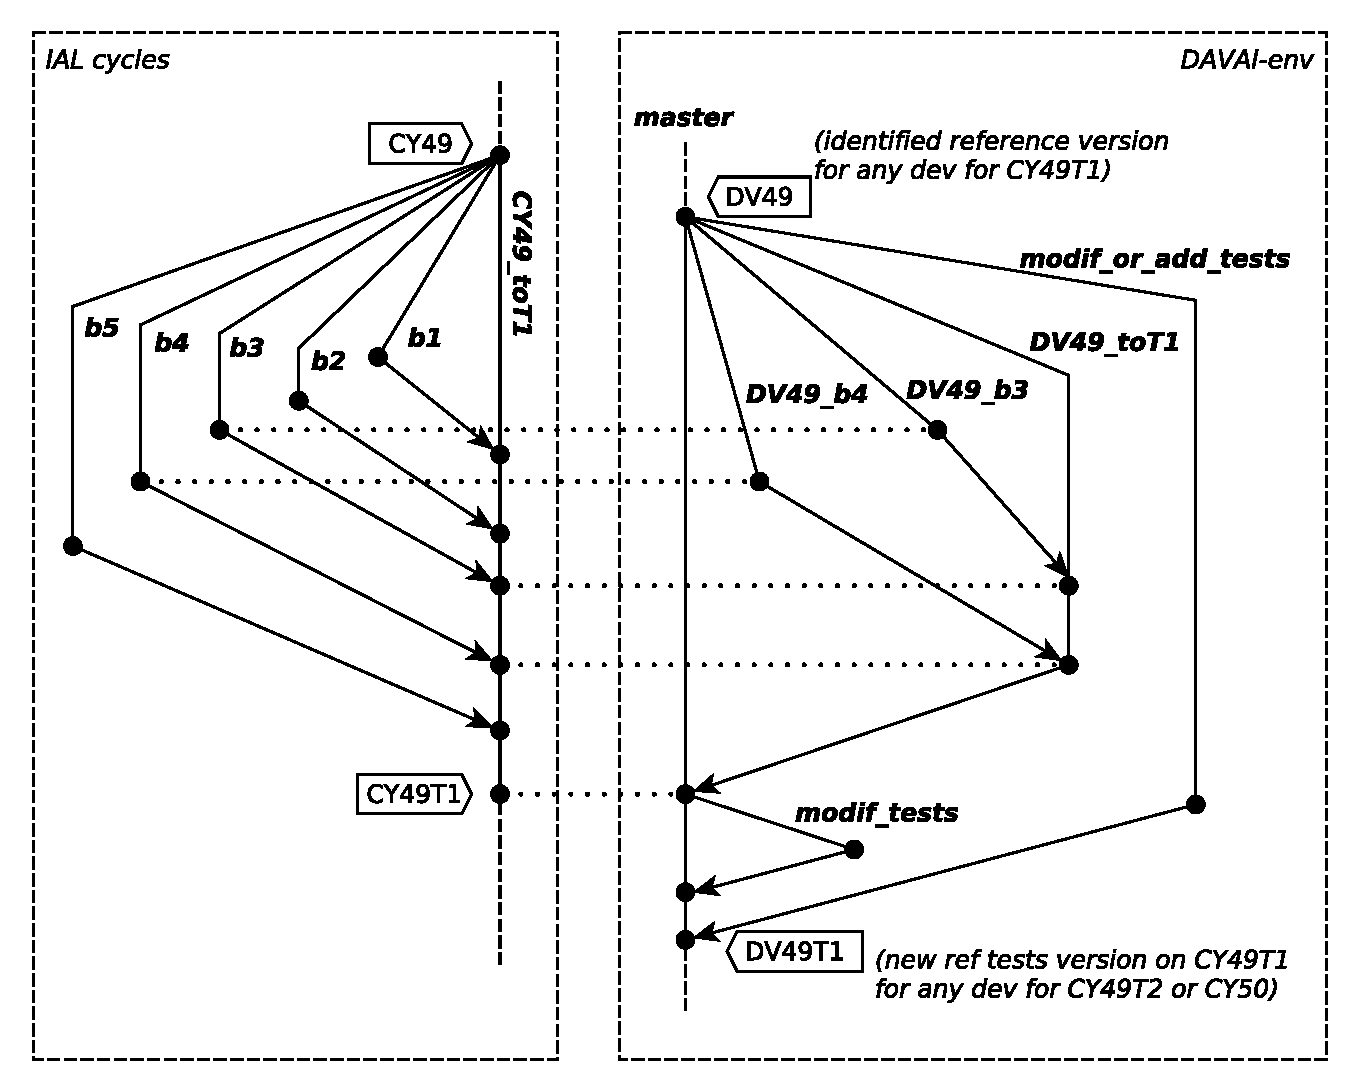
\includegraphics[scale=0.65]{../figures/tests_versioning.pdf}}
 \end{center}
 \caption{\label{fig:tests_versioning} Versioning of tests in consistency with cycles and branches.}
\end{figure}


\subsection{Adding or updating tests independently from the code\label{sect:add-modify-tests}}

The tests modifications which are not intrinsically linked with a contribution (adding tests or modifying a test to modify its behaviour) can be done at any moment, in a development branch of the tests repository. However, in order not to disturb the users and integrators, they should be merged into the next official version of tests (i.e. the version used for contributions and integrations to IAL) \underline{only between a declaration of an IAL release and a call for contribution}.


\subsection{Evolution of the tests w.r.t. Integration of an IAL release\label{sect:parallel-branches}}

In the context of integration of an IAL release, it is suitable that the tests change as little as possible during the successive integration of contributions. Therefore we will set a version of the tests at the beginning of integration, and only adapt it for the contributions that require an update of the tests.\\

Let's consider the process of integration of contribution branches on top of \texttt{CY49} to build a \texttt{CY49T1}.
For that purpose we would have set a reference experiment on \texttt{CY49}, hereafter named \texttt{x0}, generated with an identified version of the tests. That version of the tests would then be updated with \texttt{x0} as \textit{reference experiment} (\texttt{ref\_xpid}), and tagged \texttt{DV49}.
All contributions to \texttt{CY49T1} would then be required to be tested with this version \texttt{DV49} (hence against reference experiment \texttt{x0}). Cf. section~\ref{sect:set_a_ref_tests_version} for more details about setting up a reference tests version and experiment.

Suppose then that we have 5 of these contribution branches based on \texttt{CY49}, and an integration branch named \texttt{dev\_CY49\_toT1}. These 4 contributions may have different levels of reproducibility: they may conserve the results or not; they may require resources/tests adaptations (e.g. namelist updates, ...) or not, in which case they come with tests adaptations in an associated tests branch. Cf. the table :\\

\begin{center}
\begin{tabular}{|c|c|c|c|l|c|}
\hline
 branch & results & test XPID & resources & tested with & integration XPID\\
 \hline
 \texttt{b1} & $=$ & \texttt{x1} & $=$ & \texttt{DV49} & \texttt{xi1}\\
 \texttt{b2} & $\neq$ & \texttt{x2} & $=$ & \texttt{DV49} & \texttt{xi2}\\
 \texttt{b3} & $=$ & \texttt{x3} & $\neq$ & $\rightarrow$ \texttt{DV49\_b3} & \texttt{xi3}\\
 \texttt{b4} & $\neq$ & \texttt{x4} & $\neq$ & $\rightarrow$ \texttt{DV49\_b4} & \texttt{xi4}\\
 \hline
\end{tabular}
\end{center}

\noindent In parallel to the integration branch \texttt{dev\_CY49\_toT1}, we start a tests branch from \texttt{DV49} to collect the necessary adaptations of the tests, similarly named \texttt{dev\_DV49\_toT1}, which will be used to validate the integration branch, and updated as required along the integration.

In case some intermediate versions of the integration branch are tagged and some branches are based/rebased on these tagged versions, we could also tag accordingly the tests branch if necessary.\\

The reference experiment for the integration branch is at any moment, \textit{by default}, the experiment which tested the formerly integrated branch, e.g. the reference for \texttt{xi2} is \texttt{xi1}. However, that may not be true in some cases, some of these being potentially more tricky to validate, as will be shown in the following example.

\subsubsection{Steps and updates in the Continuous Integration process}
\begin{enumerate}[label=(\arabic*)]
 \item Integration of \texttt{b1} :
 \begin{itemize}
  \item Reference: \texttt{x0} is the default reference xp in \texttt{dev\_DV49\_toT1} config file
  \item Tests: \texttt{b1} did not require to adapt the tests $\rightarrow$ we can test with branch \texttt{dev\_DV49\_toT1} unchanged (and still equal to \texttt{DV49})
 \end{itemize}
 \texttt{davai-new\_xp dev\_CY49\_toT1 -v dev\_DV49\_toT1}\\
 $~~~\hookrightarrow~~~$ \texttt{xi1 == x1 == x0}

 \item Integration of \texttt{b2} :
 \begin{itemize}
  \item Reference: \texttt{xi1} should normally be the reference xp, but since its results are bit-identical to \texttt{x0} as opposed to \texttt{x2}, it is more relevant to compare to \texttt{x2}, to check that the merge of \texttt{b1} and \texttt{b2} still give the same results as \texttt{b2}
  \item Tests: \texttt{b2} did not require to adapt the tests $\rightarrow$ tests branch \texttt{DV49\_toT1} unchanged
 \end{itemize}
 \texttt{davai-new\_xp dev\_CY49\_toT1 -v DV49\_toT1}\\
 $~~~$and set \texttt{ref\_xpid = x2}\\
 $~~~\hookrightarrow~~~$ \texttt{xi2 == x2}
 \begin{itemize}
  \item then \texttt{ref\_xpid} should be set to \texttt{xi2} in branch \texttt{DV49\_toT1}
 \end{itemize}

 \item Integration of \texttt{b3} :
 \begin{itemize}
  \item Reference: \texttt{b3} does not change the results, so reference experiment is as expected by default \texttt{xi2}
  \item Tests: \texttt{b3} requires tests adaptations (\texttt{DV49\_b3}) $\rightarrow$ update \texttt{dev\_DV49\_toT1} by merging \texttt{DV49\_b3} in
 \end{itemize}
 \texttt{davai-new\_xp dev\_CY49\_toT1 -v DV49\_toT1}\\
 $~~~\hookrightarrow~~~$ \texttt{xi3 == xi2}
 
 \item Integration of \texttt{b4} : \textit{(where it becomes more or less tricky)}
 \begin{itemize}
  \item Reference: \texttt{b4} changes the results, but the results of \texttt{xi3} (current default reference for integration branch) are also changed from \texttt{x0} (since \texttt{b2}) $\rightarrow$ the reference experiment becomes less obvious !\\
  The choice of the reference should be made depending on the width of impact on both sides:
  \begin{enumerate}[label=\alph*)]
   \item if there is more differences in the results between \texttt{dev\_CY49\_toT1} and \texttt{CY49} than between \texttt{b4} and \texttt{CY49}:\\
   $\rightarrow$ \texttt{xi3} should be taken as reference, and the differences finely compared to those shown in \texttt{x4}
   \item if there is more differences in the results between \texttt{b4} and \texttt{CY49} than between \texttt{dev\_CY49\_toT1} and \texttt{CY49}:\\
   $\rightarrow$ \texttt{x4} should be taken as reference, and the differences finely compared to those shown in \texttt{xi3'}, where \texttt{xi3'} is a \textit{``witness''} experiment comparing the integration branch after integration of \texttt{b3} (commit \texttt{<c3>}) to \texttt{CY49} (experiment \texttt{x0}):\\
   \texttt{davai-new\_xp <c3> -v dev\_DV49\_toT1}\\
   $~~~$and set \texttt{ref\_xpid = x0}\\
   $~~~\hookrightarrow~~~$ \texttt{xi3'}
  \end{enumerate}
  This is still OK if the tests affected by \texttt{dev\_CY49\_toT1} (via \texttt{b2}) and the tests affected by \texttt{b4} are not the same subset, or if at least if the affected fields are not the same. If they are (e.g. numerical differences that propagate prognostically through the model), the conclusion becomes much more difficult !!!\\
  In this case, we do not really have explicit recommendation; the integrators should double-check the result of the merge with the author of the contribution \texttt{b4}. Any idea welcome to sort it out.
  \item Tests: \texttt{b4} requires tests adaptations (\texttt{DV49\_b4}) $\rightarrow$ update \texttt{dev\_DV49\_toT1} by merging in \texttt{DV49\_b4} in
 \end{itemize}
 \texttt{davai-new\_xp dev\_CY49\_toT1 -v dev\_DV49\_toT1}\\
   $~~~$and set \texttt{ref\_xpid = xi3|xi4}\\
   $~~~\hookrightarrow~~~$ \texttt{xi4}
\end{enumerate}

\subsection{Setting up a reference version of the tests and an associated reference experiment\label{sect:set_a_ref_tests_version}}

[ ! WORK IN PROGRESS...]

We describe here how to set up a reference version of the tests and an associated reference experiment, typically for developments based on a given IAL release to be validated against this release.

For the example, let's consider \texttt{CY49} and setting up a \texttt{DV49} version for it, including its reference experiment, to validate the contributions to \texttt{CY49T1}.
\begin{enumerate}[label=\arabic*),start=0]
 \item Choose an initial version of the tests you want to be used. It may probably not be the previous reference one (e.g. \texttt{DV48T2} or \texttt{dev\_CY48T1\_toT2}), as we may often want to modify or add tests in between cycles.
 \item In your development DAVAI-tests repository, make a branch starting from this version and check it out, e.g.:\\
 \texttt{git checkout -b on\_49 [<chosen\_initial\_ref]}
 \item Set the reference experiment:\\
 \texttt{davai-new\_xp CY49 -v on\_49 -u ELP --origin <URL of my DAVAI-tests repo>}\\
 $\hookrightarrow$ \texttt{dv-xxxx-machine@user}\\
 Note:
 \begin{itemize}
  \item As ELP usecase encompasses NRV, reference experiments should use this usecase so it could be used as a reference for both usecases.
  \item \texttt{--origin <URL...>} to clone that repo in which you created the branch
  \item in config of the experiment, set \texttt{archive\_as\_ref = True} : the experiment will serve as a reference, so we want to archive its results
  \item in config of the experiment, set \texttt{ignore\_reference = True} : if you are confident enough with the test version, it may not be useful/relevant to compare the experiment to any reference one.
 \end{itemize}
 \item Run the experiment
 \item Update the \texttt{DAVAI-tests} repository:
 \begin{itemize}
  \item default config file for this machine (\texttt{conf/<machine>.ini}: with the name of this experiment as \texttt{ref\_xpid} (and potentially the usecase chosen in minor case as \texttt{ref\_vconf})
  \item \texttt{README.md}: the table of correspondance of branches and tests
 \end{itemize}
 Then commit, tag (\texttt{DV49}) and push:
 \begin{verbatim}
  git commit -am "Set reference experiment for <machine> as <dv-xxxx-machine@user>"
  git tag DV49
  git push <remote>
  git push <remote> DV49
 \end{verbatim}
\end{enumerate}

\noindent This way the tests experiment generated using \texttt{davai-new\_xp -v DV49} will use this version and be compared to this reference experiment.








\newpage
\section{Internal organization of DAVAÏ}

\begin{figure}[h!]\hspace{-2cm}
 \begin{center}\hspace{-2cm}
  \fbox{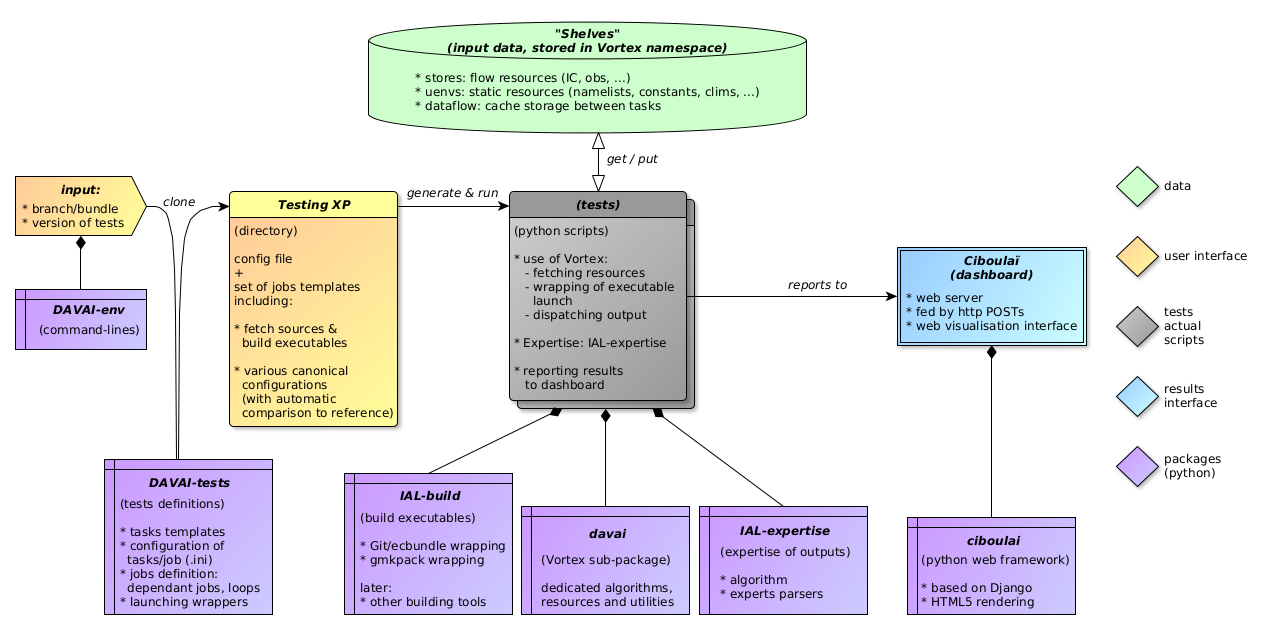
\includegraphics[scale=0.4]{../figures/davai_ecosystem_h.pdf}}
 \end{center}
 \caption{\label{fig:davai_ecosystem} DAVAI packages.}
\end{figure}



\end{appendix}
\end{document}
